\documentclass[aspectratio=169]{beamer}
\usetheme{Madrid}
\usecolortheme{seahorse}
\usepackage{graphicx}
\usepackage{booktabs}
\usepackage{xcolor}
\usepackage{tikz}
\usetikzlibrary{shapes.geometric, arrows.meta, positioning, calc}

% Custom colors
\definecolor{darkblue}{RGB}{26, 82, 118}
\definecolor{lightblue}{RGB}{174, 214, 241}
\definecolor{accentorange}{RGB}{230, 126, 34}
\definecolor{softgreen}{RGB}{39, 174, 96}
\definecolor{softred}{RGB}{192, 57, 43}

\setbeamercolor{title}{fg=darkblue}
\setbeamercolor{frametitle}{fg=darkblue,bg=lightblue!30}
\setbeamercolor{structure}{fg=darkblue}
\setbeamercolor{block title}{bg=darkblue,fg=white}
\setbeamercolor{block body}{bg=lightblue!20,fg=black}

\title[FE-NLP Group A]{Data Infrastructure \& Control Variables}
\subtitle{for S\&P 500 AI Disclosure NLP Project}
\author{Rico Zhu (Group A)}
\institute{Financial Economics Research Lab}
\date{\today}

\begin{document}

%=============================================================================
% SLIDE 1: Title
%=============================================================================
\begin{frame}
\titlepage
\end{frame}

%=============================================================================
% SLIDE 2: 10-K Data Extraction & NLP Pipeline
%=============================================================================
\begin{frame}{10-K Data Extraction \& NLP Pipeline}

\begin{columns}[T]
\begin{column}{0.55\textwidth}
\textbf{Data Sources:}
\begin{itemize}
    \item SEC EDGAR API: S\&P 500 10-K filings (FY 2019--2025)
    \item WRDS Compustat: Annual fundamentals
    \item WRDS CRSP: Monthly stock returns
    \item WRDS IBES: Analyst EPS forecasts
\end{itemize}

\vspace{0.3cm}
\textbf{NLP Pipeline Architecture:}
\begin{enumerate}
    \item \textbf{Extraction:} Download 10-K HTML, parse MD\&A section
    \item \textbf{Segmentation:} Split MD\&A into $\sim$1.96M sentences
    \item \textbf{Pre-filtering:} AI keyword detection ($\sim$3,580 candidates)
    \item \textbf{LLM Classification:} Kimi CLI / OpenAI API concurrent workers
\end{enumerate}
\end{column}

\begin{column}{0.42\textwidth}
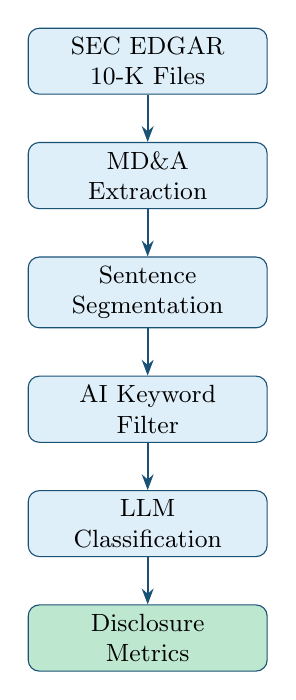
\begin{tikzpicture}[
    node distance=0.6cm,
    box/.style={rectangle, rounded corners, draw=darkblue, fill=lightblue!40, 
                text width=2.8cm, minimum height=0.7cm, align=center, font=\small},
    arrow/.style={-{Stealth[length=2mm]}, thick, darkblue}
]
\node[box] (edgar) {SEC EDGAR\\10-K Files};
\node[box, below=of edgar] (mdna) {MD\&A\\Extraction};
\node[box, below=of mdna] (sent) {Sentence\\Segmentation};
\node[box, below=of sent] (filter) {AI Keyword\\Filter};
\node[box, below=of filter] (llm) {LLM\\Classification};
\node[box, below=of llm, fill=softgreen!30] (out) {Disclosure\\Metrics};

\draw[arrow] (edgar) -- (mdna);
\draw[arrow] (mdna) -- (sent);
\draw[arrow] (sent) -- (filter);
\draw[arrow] (filter) -- (llm);
\draw[arrow] (llm) -- (out);
\end{tikzpicture}
\end{column}
\end{columns}

\vspace{0.3cm}
\begin{block}{Key Output}
\texttt{firm\_year\_ai\_disclosure\_summary.csv}: 3,359 firm-years with 5 AI disclosure intensity measures
\end{block}

\end{frame}

%=============================================================================
% SLIDE 3: Control Variable Database
%=============================================================================
\begin{frame}{Control Variable Database: From Raw to Regression-Ready}

\textbf{WRDS Data Integration:}
\begin{itemize}
    \item \textbf{Compustat:} 60,689 firm-years, 10,497 firms (FY 2018--2025)
    \item \textbf{CRSP:} Monthly returns for momentum \& volatility (80.3\% coverage)
    \item \textbf{IBES:} FY1/FY2 EPS consensus forecasts ($\sim$93\% coverage)
\end{itemize}

\vspace{0.2cm}
\textbf{Critical Data Cleaning Challenges:}
\begin{table}
\centering
\small
\begin{tabular}{@{}lll@{}}
\toprule
\textbf{Issue} & \textbf{Example} & \textbf{Fix} \\
\midrule
Ticker mismatch & BRK-B $\neq$ BRK.B & Map before merge \\
Fiscal year misalignment & WMT FYE Jan 2020 & Adjust fyear $-1$ \\
Dual-class duplicates & GOOG/GOOGL same 10-K & Keep primary class \\
gvkey zero-padding & ``1004'' vs ``001004'' & \texttt{str.zfill(6)} \\
\bottomrule
\end{tabular}
\end{table}

\vspace{0.2cm}
\textbf{Derived Variables:}
\begin{columns}[T]
\begin{column}{0.48\textwidth}
\begin{itemize}
    \item Future performance (t+1): \texttt{future\_ROA}, \texttt{future\_sales\_growth}
    \item Winsorized ratios: \texttt{tobin\_q\_winsorized}, \texttt{leverage\_winsorized}
    \item Market variables: \texttt{momentum\_12m}, \texttt{volatility\_12m}
\end{itemize}
\end{column}
\begin{column}{0.48\textwidth}
\begin{itemize}
    \item Industry FE: \texttt{sic}, \texttt{naics}, \texttt{gsubind}, \texttt{sector}
    \item Time FE: \texttt{fyear}, \texttt{post\_ai} (GenAI boom dummy)
    \item Disclosure dummies: \texttt{has\_substantive\_ai}, etc.
\end{itemize}
\end{column}
\end{columns}

\end{frame}

%=============================================================================
% SLIDE 4: Final Panel & Regression Support
%=============================================================================
\begin{frame}{Final Panel \& Regression Support}

\begin{columns}[T]
\begin{column}{0.58\textwidth}
\textbf{Final Panel:} \texttt{firm\_year\_panel\_regression\_ready.csv}
\begin{itemize}
    \item 3,338 firm-years $\times$ 73 variables
    \item 7 fiscal years (2019--2025)
    \item 489 unique firms (after dual-class dedup)
\end{itemize}

\vspace{0.3cm}
\textbf{Regression Sample Flags:}
\begin{table}
\centering
\small
\begin{tabular}{@{}lcc@{}}
\toprule
\textbf{Specification} & \textbf{Obs.} & \textbf{Key Requirements} \\
\midrule
Valuation (Tobin's Q) & 1,949 & All controls + AI vars non-missing \\
Future Performance & 1,692 & + future\_ROA, future\_sales\_growth \\
Analyst Forecast & $\sim$3,120 & + IBES FY1 EPS consensus \\
\bottomrule
\end{tabular}
\end{table}

\vspace{0.3cm}
\textbf{Deliverables for Regression Team:}
\begin{itemize}
    \item Stata \texttt{.do} file with sample flags \& winsorization
    \item Python pandas merge templates
    \item Documentation: \texttt{README\_PANEL.md}
\end{itemize}
\end{column}

\begin{column}{0.40\textwidth}
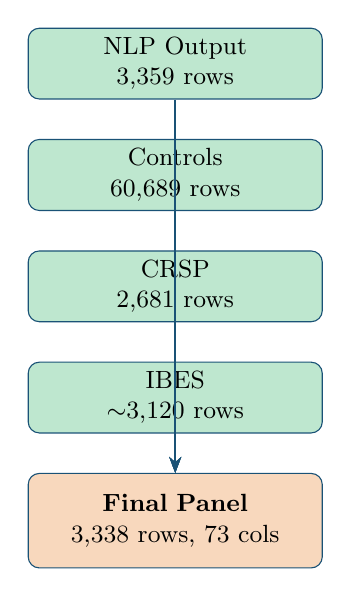
\begin{tikzpicture}[
    node distance=0.5cm,
    box/.style={rectangle, rounded corners, draw=darkblue, fill=lightblue!40, 
                text width=3.5cm, minimum height=0.8cm, align=center, font=\small},
    arrow/.style={-{Stealth[length=2mm]}, thick, darkblue}
]
\node[box, fill=softgreen!30] (nlp) {NLP Output\\3,359 rows};
\node[box, below=of nlp, fill=softgreen!30] (ctrl) {Controls\\60,689 rows};
\node[box, below=of ctrl, fill=softgreen!30] (crsp) {CRSP\\2,681 rows};
\node[box, below=of crsp, fill=softgreen!30] (ibes) {IBES\\$\sim$3,120 rows};
\node[box, below=of ibes, fill=accentorange!30, minimum height=1.2cm] (panel) {\textbf{Final Panel}\\3,338 rows, 73 cols};

\draw[arrow] (nlp) -- (panel);
\draw[arrow] (ctrl) -- (panel);
\draw[arrow] (crsp) -- (panel);
\draw[arrow] (ibes) -- (panel);
\end{tikzpicture}
\end{column}
\end{columns}

\vspace{0.3cm}
\begin{block}{Impact}
Complete data infrastructure enabling DiD, OLS, and IV regressions on AI disclosure $\rightarrow$ firm performance
\end{block}

\end{frame}

\end{document}
